\documentclass{article}

\title{\sc\LARGE CSCA67 Tutorial, Week 2\\
{\Large Sept. 21st-25th, 2015}}
\date{}
\author{\sc Compiled by {\em G. Singh Cadieux}\\[1ex]
\sc Adapted from\\
A. Bretscher, \href{http://www.utsc.utoronto.ca/~bretscher/a67/lectures/w2.pdf}{\em CSCA67 Week 2 Lecture Notes},\\
\href{http://www.intmath.com/counting-probability/3-permutations.php}{\em Interactive Mathematics: Permutations (Ordered Arrangements)},\\
\href{http://www.intmath.com/counting-probability/4-combinations.php}{\em Interactive Mathematics: Combinations (Unordered Selections)},\\
Hunter, David J. \textit{Essentials of Discrete Mathematics.} Jones \& Bartlett, 2012. \&\\
Lov\'{a}sz, et al. \textit{Discrete Mathematics: Elementary and Beyond.} Springer, 2003.}

\usepackage{fullpage}
\usepackage{amsmath,amssymb}
%\usepackage{color}
%\usepackage{multicol}
\usepackage{tikz}
\usepackage{hyperref}

\setlength{\parindent}{0pt}

\begin{document}
\maketitle

\section{\sc Review of week 2's lecture}
\subsection{\em Sum rule vs. product rule}
\begin{tabular}{p{0.5\textwidth}|p{0.5\textwidth}}
{\bf Sum Rule}&{\bf Product Rule}\\[0.5ex]\hline\hline\noalign{\smallskip}
Used for counting the \textbf{total \# of possible outcomes} of an operation which can be performed $n$ ways, each with some number of outcomes.&
Used for counting the \textbf{total \# of possible ways} an operation can be performed when the operation takes $k$ steps, each of which can be performed in some number of ways.\\\hline
\begin{equation*}
\sum\limits_{i=1}^n x_i
\end{equation*}
where way $i$ has $x_i$ possible outcomes.&
\begin{equation*}
\prod\limits_{i=1}^k x_i
\end{equation*}
where step $k$ can be performed in $x_i$ ways.\\\hline\noalign{\smallskip}
\multicolumn{2}{c}{\em From Week 1's pizza example:}\\\hline\noalign{\smallskip}
Used for counting the number of combinations of up to 5 pizza toppings.\newline
Recall:\newline
\# of combinations of up to 5 toppings =
\begin{flushright}
\# of combinations of no toppings +\\
\# of combinations of 1 topping +\\
\ldots +\\
\# of combinations of 5 toppings
\end{flushright}
&
Used for counting the number of combinations of 5 pizza toppings (and 4, 3, etc.).\newline
Recall:\newline
\# of (non-unique) combinations of 5 toppings =
\begin{flushright}
\# of ways to choose first topping $\times$\\
\# of ways to choose second topping $\times$\\
\ldots $\times$\\
\# of ways to choose fifth topping
\end{flushright}
\end{tabular}

\subsection{\em Permutation vs. combination}
\begin{tabular}{c|c}
{\bf Permutation}&{\bf Combination}\\[0.5ex]\hline\hline\noalign{\smallskip}
\textit{Ordered} arrangement of a group of objects.& \textit{Unordered} arrangement of a group of objects.\\[0.5ex]\hline\noalign{\smallskip}
Total \# of permutations of $n$ objects: $n!$&Total \# of combinations of $n$ objects: 1\\[0.5ex]\hline\noalign{\smallskip}
{\bf $r$-permutation:}&{\bf $r$-combination:}\\
permutation of $r$ objects from a group of $n$ objects&combination of $r$ objects from a group of $n$ objects\\[1ex]
Total \# of $r$-permutations: $\dfrac{n!}{(n-r)!}$&Total \# of $r$-combinations: $\dfrac{n!}{(n-r)!\,r!}$\\[0.5ex]\noalign{\smallskip}\hline\noalign{\smallskip}
Represented $P(n,r)$&Represented $C(n,r)$ or $\binom{n}{r}$
\end{tabular}\\[2ex]
\textsc{Consider first} the number of permutations of $n$ objects.\\[1ex]
This is equivalent to considering the number of ways we can arrange $n$ objects. We can see that this will require $n$ steps: the first step is selecting the first object in the arrangement; the second step is selecting the second object, and so on.\\[1ex]
Using the product rule, we determine that
\begin{multline*}
\text{\bf\# of ways of permuting }n\text{ \bf objects}=\text{\# of ways of selecting the first object }\times\\
\text{\# of ways of selecting the second object }\times\ldots\times\text{\# of ways of selecting the }n\text{th object}
\end{multline*}
When we select the first object, there are $n$ objects from which to choose, meaning that there are $n$ ways to select an object. When we select the second object, we select from the reduced group of $(n-1)$ objects, since we have already selected one; this means that there are $(n-1)$ ways to choose. Eventually, when we select the final, $n$th object, we select from a group of only 1 object, which can only be done in 1 way.\\[1ex]
Overall, we can see that
\begin{equation*}
\text{\# of ways of permuting }n\text{ objects}=n\times(n-1)\times\ldots\times 1=n!
\end{equation*}
\textsc{Using this result,} we can determine the number of $r$-permutations of $n$ objects.\\[1ex]
If we select a subset of $r$ objects from an overall group of $n$ objects, we ignore the remaining $(n-r)$ objects.\\[1em]
Consider the 2-permutations of \{A, B, C, D, E\}.\\[1ex]
If we select \{A, B\}, we have 2 possible 2-permutations: AB and BA. We can permute all 5 objects to obtain (among others) ABCDE, ABCED, and ABDEC. However, because we have selected only \{A, B\} to permute, and ABCDE, ABCED, and ABDEC contain the same permutation AB of \{A, B\}, these 3 are equivalent here.\\[1ex]
To determine the number of 2-permutations, we can diminish the number of 5-permutations (permutations of all 5 objects) by the number of 5-permutations we consider to be equivalent.\\[1ex]
Having selected 2 ordered objects, the remaining 3 objects can be permuted $3!$ times: by the same reasoning as above, we can select the third object from 3 in 3 ways; then we can select the fourth object from 2 in 2 ways; and finally, we can select the fifth object from the remaining 1 object in only 1 way.\\
Since we are interested only in the order of the first 2 objects we selected, there are $3!$ ways that the remaining 3 objects can be selected to produce permutations we consider equivalent. So of the $5!$ total 5-permutations, we consider only 1 out of $3!$ to be a unique 2-permutation.\\
And thus, there are $\dfrac{5!}{3!}=20$ 2-permutations of \{A, B, C, D, E\}.\\[1em]
We can generalize this to say that
\begin{equation*}
\text{total \# of }r\text{-perms.}=\dfrac{\text{total \# of perms. of }n\text{ objects}}{\text{total \# of perms. of the remaining }(n-r)\text{ objects}}=\dfrac{n!}{(n-r)!}
\end{equation*}\\[1em]
\textsc{We can use this result} to determine the number of $r$-combinations of $n$ objects.\\[1ex]
Unlike an $r$-permutation, an $r$-combination is unordered. From all possible $r$-permutations of $n$ objects, we have multiple equivalent $r$-combinations.\\[1em]
Consider again the 2-permutations of \{A, B, C, D, E\}.\\[1ex]
If we select \{A, B\}, we have 2 possible 2-permutations: AB and BA. However, these are equivalent $r$-combinations, since both are composed of the same objects. For every possible 2-permutation \{object1, object2\}, there is another 2-permutation \{object2, object1\} that contains the same objects in the reverse order.\\[1ex]
To determine the number of 2-combinations, we can diminish the total number of 2-permutations by the number of 2-permutations which contain the same group of 2 objects.\\
Here, there are $\dfrac{5!}{3!}\dfrac{1}{2}=\dfrac{20}{2}=10$ 2-combinations of \{A, B, C, D, E\}.\\[1em]
We can generalize this to say that, in a group of $n$ objects, the number of $r$-permutations containing the same group of $r$ objects is $r!$, the number of ways that $r$ objects can be ordered. So of the $\dfrac{n!}{(n-r)!}$ total $r$-permutations, only 1 out of $r!$ is a unique $r$-combination.
\begin{equation*}
\text{total \# of }r\text{-combs.}=\dfrac{\text{total \# of }r\text{-perms. of }n\text{ objects}}{\text{total \# of perms. of the selected }r\text{ objects}}=\dfrac{n!}{(n-r)!\,r!}
\end{equation*}

\subsection{\em Permutation with repetition}
Consider the group of letters that form the word ``banana": \{b, a, n, a, n, a\}.\\[1ex]
\textsc{Q: How many ways can we ``arrange" (here, permute) these letters?}\\[1em]
If all 6 letters were distinct, we know that there would be $6!$ arrangements. We come to this total by multiplying together the 6 ways to choose the first letter from 6 possibilities, and the 5 ways to choose the second letter from 5 possibilities, and so on.\\[1ex]
But because the letters here are not unique, there are fewer than 6 different ways to choose the first letter, and fewer than 5 different ways to choose the second, and so on.\\[1em]
\textsc{Suppose} that we convert this to a problem in which all the letters are distinct: \{b, a$_1$, n$_1$, a$_2$, n$_2$, a$_3$\}.\\[1ex]
Then the arrangements ``ba$_1$a$_2$a$_3$n$_1$n$_2$", ``ba$_1$a$_2$a$_3$n$_2$n$_1$", and ``ba$_1$a$_3$a$_2$n$_1$n$_2$" are distinct. But without the distinguishing subscripts - that is, where all `a's are considered equivalent and all `n's are considered equivalent - these arrangements are not distinct.\\[1ex]
We can re-order equivalent letters to form equivalent arrangements.\\
For example, we can form the same arrangement ``baanna" by ordering the `a's and `n's as ``ba$_1$a$_2$n$_1$n$_2$a$_3$", ``ba$_1$a$_2$n$_2$n$_1$a$_3$", ``ba$_1$a$_3$n$_1$n$_2$a$_2$", and ``ba$_2$a$_3$n$_1$n$_2$a$_1$", among other ways. What differs between these is the order of the equivalent letters, but not their overall position in the arrangement.\\[1ex]
Thus, the total number of equivalent arrangements is the total number of ways we can order the equivalent letters: we can order 3 `a's in $3!$ ways, and 2 `n's in $2!$ ways. Then, by the product rule, we can order both `a's and `n's in $3!\times 2!$ ways.
\begin{equation*}
\text{total \# of distinct arrangements}=\dfrac{\text{total \# of arrangements}}{\text{\# of equivalent arrangements}}=\dfrac{6!}{3!\,2!}=60
\end{equation*}

\textsc{Alternatively,} rather than constructing an arrangement by selecting the first letter of the arrangement, followed by the second letter, and so on, let us select one letter out of the group and assign it a place within the arrangement. Then, we select another letter from the group and assign it one of the remaining places in the arrangement. We continue this until all the letters from the group have been placed into the arrangement. For example,
\begin{center}
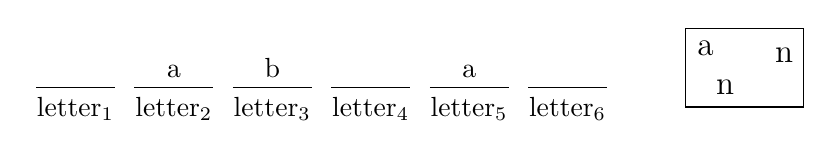
\begin{tikzpicture}
\draw (0,0) -- (0.5,0) node[below,align=center] {letter$_1$} -- (1,0);
\draw (1.25,0) -- (1.75,0) node[below,align=center] {letter$_2$} -- (2.25,0);
\draw (2.5,0) -- (3,0) node[below,align=center] {letter$_3$} -- (3.5,0);
\draw (3.75,0) -- (4.25,0) node[below,align=center] {letter$_4$} -- (4.75,0);
\draw (5,0) -- (5.5,0) node[below,align=center] {letter$_5$} -- (6,0);
\draw (6.25,0) -- (6.75,0) node[below,align=center] {letter$_6$} -- (7.25,0);
\node[above,align=center] at (1.75,0) {a};
\node[above,align=center] at (3,0) {b};
\node[above,align=center] at (5.5,0) {a};
\node[font=\large] at (8.5,0.5) {a};
\node[font=\large] at (9.5,0.4) {n};
\node[font=\large] at (8.75,0) {n};
\draw (8.25,-0.25) rectangle (9.75,0.75);
\end{tikzpicture}
\end{center}
Then, the total number of possible arrangements is the product of the number of places possible for the first letter selected, and the number of places possible for the second letter selected, and so on.\\[1ex]
If all 6 letters are distinct, then this gives us 6 possible places for the first letter, 5 possible places for the second, and so on, which is $6!$ in total, as expected.\\[1ex]
However, because the letters here are not all distinct, if we assign one letter to letter$_1$ and another instance of that letter to letter$_3$, this is equivalent to having first assigned that letter to letter$_3$ and then, another instance of it to letter$_1$. Yet we counted fewer possible places for the first assignment than the second assignment.\\[1ex]
To deal with these equivalences, we assign places to all identical letters simultaneously; that is, we assign places to all 3 `a's simultaneously, and to both `n's simultaneously.\\[1ex]
For example, this means that the number of possible places for `n's is $\dbinom{\text{\# of unassigned places}}{2}$.\\
Note that this is no different if the letters are all distinct: $\binom{6}{1}\binom{5}{1}\binom{4}{1}\binom{3}{1}\binom{2}{1}\binom{1}{1}=6\times 5\times 4\times 3\times 2\times 1=6!$.\\[1ex]
Thus, by this reasoning,
\begin{align*}
\text{total \# of distinct arrangements}& =\dbinom{\text{\# of unass. places}}{\text{\# of `a's}}\dbinom{\text{\# of unass. places}}{{\text{\# of `n's}}}\dbinom{\text{\# of unass. places}}{{\text{\# of `b's}}}\\
& =\dbinom{6}{3}\dbinom{6-3}{2}\dbinom{6-3-2}{1}\\
& =\dfrac{6!}{(6-3)!\,3!}\dfrac{3!}{(3-2)!\,2!}\dfrac{1!}{(1-1)!\,1!}\\
& =\dfrac{6!}{3!\,2!\,1!}=60
\end{align*}

\textsc{In general,} there are
\begin{equation*}
\dbinom{n}{r_1}\dbinom{n-r_1}{r_2}\ldots\dbinom{n-r_1-r_2-\ldots-r_{m-1}}{r_m}=\dfrac{n!}{r_1!\,r_2!\,\ldots\,r_m!}
\end{equation*}
distinct arrangements/permutations of $n$ objects divided into $m$ types, where $r_i$ is the number of objects of type $i=1,2,\ldots,m$.\\[1ex]
Note that the $n$ objects are \textit{partitioned} into $m$ types; that is, $r_1+r_2+\ldots+r_m=n$.

\subsection{\em Combination/selection with repetition}

Consider a situation in which a supermarket has 3 kinds of bagels: poppy seed, sesame seed, and plain.\\[1ex]
\textsc{Q: If you want to buy 6 bagels, how many combinations of different kinds can you get?}\\[1ex]
If we were selecting 6 bagels from a group of $n$ unique bagels, we know that there would be $\dbinom{n}{6}=\dfrac{n!}{(n-6)!\,6!}$ possible combinations.\\[1ex]
But because we are selecting 6 bagels \textit{with repetition} (we have only 3 types from which to choose, so we must have more than 1 of at least 1 type of bagel), some of these $\binom{n}{6}$ combinations are equivalent.\\[1ex]
For example, suppose that we convert this to a problem in which all the bagels are unique. Then the combinations
\begin{center}
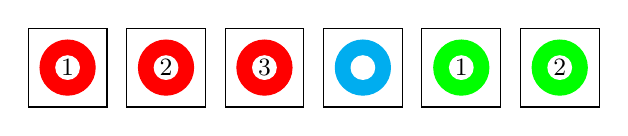
\begin{tikzpicture}
\draw (0,0) rectangle (1,1);
\draw (1.25,0) rectangle (2.25,1);
\draw (2.5,0) rectangle (3.5,1);
\draw (3.75,0) rectangle (4.75,1);
\draw (5,0) rectangle (6,1);
\draw (6.25,0) rectangle (7.25,1);

\filldraw[red] (0.5,0.5) circle (0.35);
\filldraw[white] (0.5,0.5) circle (0.15);

\filldraw[red] (1.75,0.5) circle (0.35);
\filldraw[white] (1.75,0.5) circle (0.15);

\filldraw[red] (3,0.5) circle (0.35);
\filldraw[white] (3,0.5) circle (0.15);

\filldraw[cyan] (4.25,0.5) circle (0.35);
\filldraw[white] (4.25,0.5) circle (0.15);

\filldraw[green] (5.5,0.5) circle (0.35);
\filldraw[white] (5.5,0.5) circle (0.15);

\filldraw[green] (6.75,0.5) circle (0.35);
\filldraw[white] (6.75,0.5) circle (0.15);

\node [font=\small] at (0.5,0.5) {1};
\node [font=\small] at (1.75,0.5) {2};
\node [font=\small] at (3,0.5) {3};

\node [font=\small] at (5.5,0.5) {1};
\node [font=\small] at (6.75,0.5) {2};
\end{tikzpicture}\\
and\\[1ex]
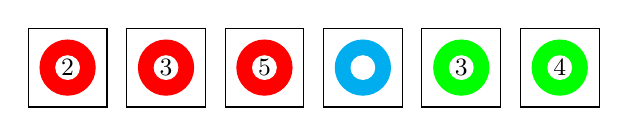
\begin{tikzpicture}
\draw (0,0) rectangle (1,1);
\draw (1.25,0) rectangle (2.25,1);
\draw (2.5,0) rectangle (3.5,1);
\draw (3.75,0) rectangle (4.75,1);
\draw (5,0) rectangle (6,1);
\draw (6.25,0) rectangle (7.25,1);

\filldraw[red] (0.5,0.5) circle (0.35);
\filldraw[white] (0.5,0.5) circle (0.15);

\filldraw[red] (1.75,0.5) circle (0.35);
\filldraw[white] (1.75,0.5) circle (0.15);

\filldraw[red] (3,0.5) circle (0.35);
\filldraw[white] (3,0.5) circle (0.15);

\filldraw[cyan] (4.25,0.5) circle (0.35);
\filldraw[white] (4.25,0.5) circle (0.15);

\filldraw[green] (5.5,0.5) circle (0.35);
\filldraw[white] (5.5,0.5) circle (0.15);

\filldraw[green] (6.75,0.5) circle (0.35);
\filldraw[white] (6.75,0.5) circle (0.15);

\node [font=\small] at (0.5,0.5) {2};
\node [font=\small] at (1.75,0.5) {3};
\node [font=\small] at (3,0.5) {5};

\node [font=\small] at (5.5,0.5) {3};
\node [font=\small] at (6.75,0.5) {4};
\end{tikzpicture}
\end{center}
are distinct. But without the distinguishing identifiers - that is, where all bagels of the same type are considered equivalent - these combinations are not distinct.\\[1ex]
\textsc{Since all} bagels of the same type are equivalent, rather than considering how to select 6 bagels one by one for the arrangement, let us consider how to divide our arrangement into 3 groups of types of bagels.\\
For example, we can divide our 6 possibilities into a group of 1 poppy seed bagel, a group of 4 sesame seed bagels, and a group of 1 plain bagel:
\begin{center}
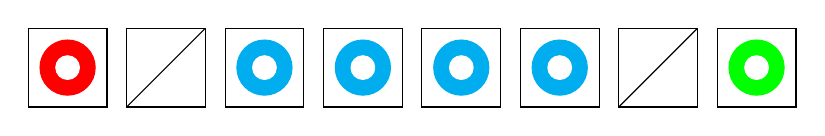
\begin{tikzpicture}
\draw (0,0) rectangle (1,1);
\draw (1.25,0) rectangle (2.25,1);
\draw (2.5,0) rectangle (3.5,1);
\draw (3.75,0) rectangle (4.75,1);
\draw (5,0) rectangle (6,1);
\draw (6.25,0) rectangle (7.25,1);
\draw (7.5,0) rectangle (8.5,1);
\draw (8.75,0) rectangle (9.75,1);

\filldraw[red] (0.5,0.5) circle (0.35);
\filldraw[white] (0.5,0.5) circle (0.15);

\filldraw[cyan] (3,0.5) circle (0.35);
\filldraw[white] (3,0.5) circle (0.15);

\filldraw[cyan] (4.25,0.5) circle (0.35);
\filldraw[white] (4.25,0.5) circle (0.15);

\filldraw[cyan] (5.5,0.5) circle (0.35);
\filldraw[white] (5.5,0.5) circle (0.15);

\filldraw[cyan] (6.75,0.5) circle (0.35);
\filldraw[white] (6.75,0.5) circle (0.15);

\filldraw[green] (9.25,0.5) circle (0.35);
\filldraw[white] (9.25,0.5) circle (0.15);

\draw (1.25,0) -- (2.25,1);
\draw (7.5,0) -- (8.5,1);
\end{tikzpicture}
\end{center}
To mark the separation between groups, we use an empty pigeonhole. To divide our bagels into 3 groups, we require 2 pigeonholes to act as separators, and 6 filled pigeonholes + 2 empty pigeonholes = 8 piegeonholes in total.\\[1ex]
\textsc{In general,} to partition any number of objects into $n$ groups, we require $n-1$ empty pigeonholes.\\[1ex]
We can divide our 6 possibilities into 3 groups by selecting which pigeonholes will be filled and which will be empty. For example, if we select all but these pigeonholes to be filled
\begin{center}
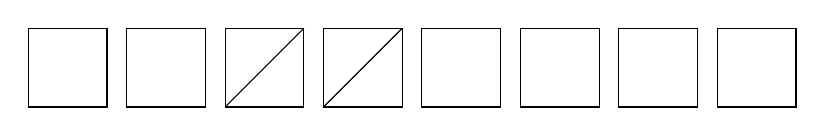
\begin{tikzpicture}
\draw (0,0) rectangle (1,1);
\draw (1.25,0) rectangle (2.25,1);
\draw (2.5,0) rectangle (3.5,1);
\draw (3.75,0) rectangle (4.75,1);
\draw (5,0) rectangle (6,1);
\draw (6.25,0) rectangle (7.25,1);
\draw (7.5,0) rectangle (8.5,1);
\draw (8.75,0) rectangle (9.75,1);

\draw (2.5,0) -- (3.5,1);
\draw (3.75,0) -- (4.75,1);
\end{tikzpicture}
\end{center}
then our groups are 2 poppy seed bagels, 0 sesame seed bagels, and 4 plain bagels:
\begin{center}
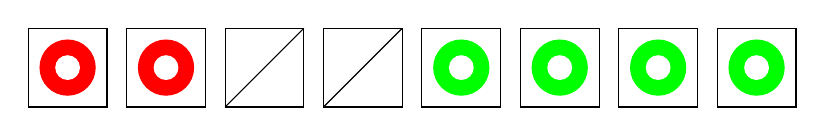
\begin{tikzpicture}
\draw (0,0) rectangle (1,1);
\draw (1.25,0) rectangle (2.25,1);
\draw (2.5,0) rectangle (3.5,1);
\draw (3.75,0) rectangle (4.75,1);
\draw (5,0) rectangle (6,1);
\draw (6.25,0) rectangle (7.25,1);
\draw (7.5,0) rectangle (8.5,1);
\draw (8.75,0) rectangle (9.75,1);

\filldraw[red] (0.5,0.5) circle (0.35);
\filldraw[white] (0.5,0.5) circle (0.15);

\filldraw[red] (1.75,0.5) circle (0.35);
\filldraw[white] (1.75,0.5) circle (0.15);

\filldraw[green] (5.5,0.5) circle (0.35);
\filldraw[white] (5.5,0.5) circle (0.15);

\filldraw[green] (6.75,0.5) circle (0.35);
\filldraw[white] (6.75,0.5) circle (0.15);

\filldraw[green] (8,0.5) circle (0.35);
\filldraw[white] (8,0.5) circle (0.15);

\filldraw[green] (9.25,0.5) circle (0.35);
\filldraw[white] (9.25,0.5) circle (0.15);

\draw (2.5,0) -- (3.5,1);
\draw (3.75,0) -- (4.75,1);
\end{tikzpicture}
\end{center}
\textsc{The question} then becomes: in how many ways can we choose our 2 empty pigeonholes, or our 6 filled pigeonholes?\\[1ex]
Since these pigeonholes are unordered, the answer is simply $\dbinom{8}{6}=28$.\\[1ex]
\textsc{In general,} there are
\begin{equation*}
\dbinom{\text{total \# of pigeonholes}}{\text{\# of objects being selected}}=\dbinom{r+(n-1)}{r}
\end{equation*}
distinct combinations of $r$ objects from a group of $n$ types of objects.

\section{\sc Counting problems: Permutations and combinations}

\subsection*{Q: {\em How many ways can the letters A, B, and C be arranged?}}
We are being asked how many different ways 3 distinct objects, the letters A, B, and C, can be permuted.\\[1ex]
There are $n!\Rightarrow 3!=6$ permutations of 3 objects.

\subsection*{Q: {\em How many ways can 4 different resistors be arranged in series?}}
Again, we are being asked how many different ways 4 distinct objects - 4 resistors - can be permuted.\\[1ex]
There are $n!\Rightarrow 4!=24$ permutations of 4 objects.

\subsection*{Q: {\em How many ways can a supermarket manager display 5 brands of cereal in 3 spaces on a shelf?}}
We are again being asked about an arrangement, or permutation, of multiple objects. However, here we must determine the number of $r$-permutations: permutations of 3 brands out of the 5 possible brands.\\[1ex]
There are $\dfrac{n!}{(n-r)!}\Rightarrow\dfrac{5!}{(5-3)!}=60$ permutations of 3 objects from 5.

\subsection*{Q: {\em How many different license plates for cars can be made if each contains 4 of the digits 0-9, followed by a letter A-Z, assuming}}
\subsubsection*{a) {\em no repetition of digits?}}
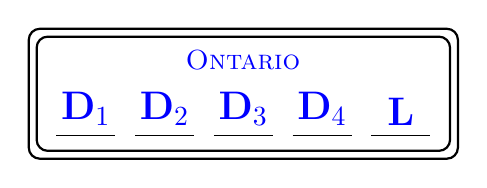
\begin{tikzpicture}
\draw[thick,rounded corners](0,0)rectangle(5.25,1.45);
\draw[thick,rounded corners](-.1,-.1)rectangle(5.35,1.55);
\node[color=blue] at (2.62,1.15) {\sc Ontario};
\draw(0.25,0.2) -- (0.625,0.2) node [align=center,above,font={\Large\bf},color=blue] {D$_1$} -- (1,0.2);
\draw(1.25,0.2) -- (1.625,0.2) node [align=center,above,font={\Large\bf},color=blue] {D$_2$} --(2,0.2);
\draw(2.25,0.2) -- (2.625,0.2) node [align=center,above,font={\Large\bf},color=blue] {D$_3$} --(3,0.2);
\draw(3.25,0.2) -- (3.625,0.2) node [align=center,above,font={\Large\bf},color=blue] {D$_4$} --(4,0.2);
\draw(4.25,0.2) -- (4.625,0.2) node [align=center,above,font={\Large\bf},color=blue] {L} --(5,0.2);
\end{tikzpicture}\\[1ex]
Let us consider all 4 digits as a single entity \textbf{D}. Then, using the multiplication principle,
\begin{align*}
\text{\# of combinations of \textbf{D} and \textbf{L}}& =\text{\# of ways of choosing \textbf{D}}\times\text{\# of ways of choosing \textbf{L}}\\
& =\text{\# of perms. of 4 digits}\times\text{\# of letters}
\end{align*}
The number of permutations of 4 digits, with no repetition of digits, is the number of 4-permutations of 10 objects, since there are 10 digits from which we select. So
\begin{align*}
\text{\# of combinations of \textbf{D} and \textbf{L}}& =\left(\dfrac{10!}{(10-4)!}\right)\times 26\\
& =5040\times 26\\
& =131\,040
\end{align*}

\subsubsection*{b) {\em possible repetition of digits?}}
If repetition of digits (using the same digit more than once) is possible, then we are no longer dealing with permutations. Instead, using the product rule, we determine that the number of ways of choosing \textbf{D} is the product of the number of ways of choosing the first digit D$_1$, and then the second digit D$_2$, and so on.\\[1ex]
Since repetition is possible, at each step, we are choosing from the same set of 10 digits, meaning that there are 10 ways to choose each digit.
\begin{align*}
\text{\# of combinations of \textbf{D} and \textbf{L}}& =\text{\# of ways of choosing \textbf{D}}\times\text{\# of ways of choosing \textbf{L}}\\
& =\left(\text{\# of ways of choosing D}_1\times\ldots\times\text{\# of ways of choosing D}_4\right)\times\text{\# of letters}\\
& =\left(10\times 10\times 10\times 10\right)\times 26\\
& =260\,000
\end{align*}

%\subsection*{Q: {\em How many different sets of 4 letters can be selected from the alphabet?}\\
%{\normalsize Eg., \{A, E, R, T\} and \{E, A, T, R\} are the same set, but are different from \{Q, D, P, T\}.}}
%We are being asked how many different ways 4 letters from the alphabet can be combined. We know that these are combinations rather than permutations because sets are, by definition, unordered.\\[1ex]
%There are $\dfrac{n!}{(n-r)!\,r!}\Rightarrow \dfrac{26!}{(26-4)!\,4!}=14\,950$ combinations of 4 objects from 26.
%
%\subsection*{Q: {\em In how many ways can 3 components be selected from a batch of 20 different components?}}
%Again, we are being asked how many different ways 3 objects from a group of 20 objects can be combined.\\[1ex]
%There are $\dfrac{n!}{(n-r)!\,r!}\Rightarrow \dfrac{20!}{(20-3)!\,3!}=1140$ combinations of 3 objects from 20.

\subsection*{Q: {\em In how many ways can a group of 4 boys be selected from 10 if}}
\subsubsection*{a) {\em the eldest boy is included in each group?}}
If the eldest boy is included in each group, we select only the remaining 3 boys in the group; and we select these other 3 group members from 9 rather than from 10, since we have already selected 1 boy.\\[1ex]
So we are asked how many different ways 3 objects can be combined from a group of 9 objects.\\[1ex]
There are $\dfrac{n!}{(n-r)!\,r!}\Rightarrow \dfrac{9!}{(9-3)!\,3!}=84$ possible groups that include the eldest boy.

\subsubsection*{b) {\em the eldest boy is excluded from all groups?}}
If the eldest boy is excluded from all groups, we select 4 boys to form a group, but we select from 9 rather than from 10, since we have eliminated 1 possible boy.\\[1ex]
There are $\dfrac{n!}{(n-r)!\,r!}\Rightarrow \dfrac{9!}{(9-4)!\,4!}=126$ possible groups that exclude the eldest boy.

\subsubsection*{c) {\em What proportion of all possible groups contain the eldest boy?}}
Since there are only two possibilities - either a group includes the eldest boy or it does not - and both possibilities cannot be true simultaneously - a group cannot simultaneously include \textit{and} exclude the eldest boy - the total number of possible groups must be the sum of the number of groups that include the eldest boy and the number of groups that do not.
\begin{align*}
\text{total \# of possible groups}& =\text{\# of groups incl. the eldest boy}+\text{\# of groups excl. the eldest boy}\\
& =84+126\\
& =210
\end{align*}
Alternatively, we can calculate the total number of possible groups as the total number of combinations of 4 boys from 10, with no restrictions:
\begin{equation*}
\text{total \# of possible groups}=\dfrac{10!}{(10-4)!\,4!}=210
\end{equation*}
The proportion of groups containing the eldest boy is then
\begin{equation*}
\dfrac{\text{\# of groups incl. the eldest boy}}{\text{total \# of possible groups}}=\dfrac{84}{210}=40\%
\end{equation*}

\section{\sc Counting problems with repetition}

\subsection*{Q: {\em How many different ways can the letters of the word ``mammal" be arranged?}}
This question is directly analogous to the ``banana" example above: we want to determine the number of arrangements of a group of objects, where some objects are of the same type.\\[1ex]
Specifically, we have $n=6$ letters, $r_1=3$ of which are `m's, $r_2=2$ of which are `a's, and $r_3=1$ of which are `l's.
\begin{equation*}
\dfrac{n!}{r_1!\,r_2!\,r_3!}\Rightarrow\dfrac{6!}{3!\,2!\,1!}=60\text{ ways to arrange ``mammal"}
\end{equation*}

\subsection*{Q: {\em How many different ways can 3 red, 4 yellow, and 2 blue bulbs be arranged in a string of Christmas lights with 9 sockets?}}
Again, we are asked to determine the number of arrangements of a group of objects with repetition.\\[1ex]
We have $n=9$ bulbs, $r_1=3$ of which are red, $r_2=4$ of which are yellow, and $r_3=2$ of which are blue.
\begin{equation*}
\dfrac{n!}{r_1!\,r_2!\,r_3!}\Rightarrow\dfrac{9!}{3!\,4!\,2!}=1260\text{ ways to arrange bulbs in 9 sockets}
\end{equation*}
\textsc{Note} that we are able to use the formula for calculating the number of arrangements with repetition, derived above, because we are asked to arrange 9 objects (in 9 sockets) and have $3+4+2=9$ objects in total.\\
That is,
\begin{equation*}
r_1+r_2+\ldots+r_m=3+4+2=9=n
\end{equation*}

%\subsection*{{\normalsize You want to send postcards to 12 friends. In the shop, there are only 3 kinds of postcards.}\\
%Q: {\em How many ways can you send the postcards if}}
%\subsubsection*{a) {\em there is a large number of each kind, and you want to send 1 card to each friend?}}
%If we are sending 1 postcard to 12 friends, we must select 12 postcards in total. However, because there are only $n=3$ kinds of postcards, some friends will receive the same kind of card.\\
%So we are being asked how many ways we can select $r=12$ postcards, with repetition. We can determine this using the formula for selection with repetition, derived above:
%\begin{equation*}
%\binom{r+(n-1)}{r}\Rightarrow\binom{12+(3-1)}{12}=\dfrac{14!}{12!\,(14-12)!}=91\text{ ways to select 12 postcards}
%\end{equation*}
%
%\subsubsection*{b) {\em there is a large number of each kind, and you are willing to send 1 or more cards to each friend, but no one should get more than 1 of the same kind of card?}}
%We are again being asked how many ways we can select \textit{at least} 12 postcards, with repetition. We cannot send more than 3 to any friend because there are only 3 types, and so, we would be sending at least more than 1 of the same type.\\[1ex]
%The number of cards we want to select can be as few as 12 (if we only send 1 to each friend) or as many as 36 (if we send 3 to each friend). This makes it difficult to use the same method as in \textbf{(a)}. Instead, we can use the product rule:
%\begin{equation*}
%\text{\# of ways to send 1-3 cards 12 times}=\underbrace{\text{\# of ways to send 1-3 cards}}_\text{friend1}\times\ldots\times\underbrace{\text{\# of ways to send 1-3 cards}}_\text{friend12}
%\end{equation*}
%Then, using the sum rule, we determine that, for each friend,
%\begin{multline*}
%\text{\# of ways to send 1-3 cards}=\\
%\text{\# of ways to send 1 card }+\text{ \# of ways to send 2 cards }+\text{ \# of ways to send 3 cards}
%\end{multline*}
%Since we cannot have repetition when selecting 2 or 3 postcards, and there are only 3 unique postcards from which to choose, we find the number of ways to choose $r=1,2,3$ postcards from $n=3$:
%\begin{align*}
%\text{\# of ways to send 1-3 postcards}& =\binom{3}{1}+\binom{3}{2}+\binom{3}{3}\\
%& =3+3+1\\
%& =7
%\end{align*}
%And finally, we determine that
%\begin{equation*}
%\text{\bf\# of ways to send 1-3 postcards 12 times}=7^{12}=13\,841\,287\,201
%\end{equation*}
%
%\subsubsection*{c) {\em there are only 4 of each kind, and you want to send 1 card to each friend?}}
%There are 4 of 3 kinds of postcards, meaning that there are $n=12$ cards in total from which to choose.\\[1ex]
%If we suppose the order in which we select the postcards to be meaningful - that is, we send the first card we select to friend1, the second to friend2, etc. - then we are being asked to determine the number of ways in which we can select 12 cards, where some cards are of the same type.
%\begin{equation*}
%\dfrac{n!}{r_1!\,r_2!\,r_3!}\Rightarrow\dfrac{12!}{4!\,4!\,4!}=34\,650\text{ ways to send 12 postcards}
%\end{equation*}

\subsection*{Q: {\em How many solutions are there to the equation $x_1+x_2+x_3+x_4+x_5=13$ if $x_1,\ldots,x_5$ must be non-negative integers?}}
We can consider this question to be asking how many ways we can distribute 13 units among the five variables $x_1,\ldots,x_5$. (We can make the question more intuitive by imagining that, as in the example above, we have five types of bagels and want to select 13 bagels in total.)\\[1ex]
For example, the solution $x_1=4,\,x_2=0,\,x_3=5,\,x_4=1,\,x_5=3$ distributes 13 1's into the five groups:
\begin{equation*}
\underbrace{\;1\;1\;1\;1\;}_{x_1}|\underbrace{\;}_{x_2}|\underbrace{\;1\;1\;1\;1\;1\;}_{x_3}|\underbrace{\;1\;}_{x_4}|\underbrace{\;1\;1\;1\;}_{x_5}
\end{equation*}
Note that a unique solution is a set of assignments to $x_1,\ldots,x_5$: thus, $x_1=4,\,x_2=0,\,x_3=5,\,x_4=1,\,x_5=3$ is a different solution than $x_1=5,\,x_2=1,\,x_3=3,\,x_4=4,\,x_5=0$.
\begin{equation*}
\binom{r+(n-1)}{r}\Rightarrow\binom{13+(5-1)}{13}=\dfrac{17!}{13!\,(17-13)!}=2380\text{ unique solutions}
\end{equation*}

\section{\sc Additional practice problems}

At a competition of 100 athletes, only the order of the first 10 is recorded.\\
{\bf Q: How many different outcomes does the competition have?}\\[1ex]
Suppose we record the order of all 100 athletes.\\
{\bf Q: How many different outcomes can we have then?}\hfill(1)\\[1ex]
{\bf Q: How many of the outcomes in {\normalfont(1)} give the same result for the first 10 places?}\hfill(2)\\[1ex]
{\bf Q: Show that the number of outcomes for the first 10 places can also be obtained using {\normalfont(1)} and {\normalfont(2)}.}\\[1em]
Possible grades for a class are A, B, C, D, and F. (No +/-'s).\\
{\bf Q: How many ways are there to assign grades to a class of seven students?}\\[1ex]
{\bf Q: How many ways are there to assign grades to a class of seven students, if nobody receives an F and exactly one person receives an A?}\\[1em]
{\bf Q: How many ways are there to arrange the letters in the word ``inaneness"?}\\[1em]
Two teams, A and B, play a best-of-seven match. The match ends when one team wins four games.\\
{\bf Q: How many different win or loss scenarios are possible?}

\end{document}